\documentclass{beamer}
\usetheme{Madrid}
\usecolortheme{beaver}
\title{Mass \& Balance}
\subtitle{Lesson 1}
\author{Alberto Botto Poala}
\institute{AeC Biella}
\date{\today}

\begin{document}

\begin{frame}
\titlepage
\end{frame} 

\begin{frame}
\frametitle{Table of Contents}
\tableofcontents
\end{frame} 

\section{Massa vs Forza Peso}
\begin{frame}
\frametitle{Title}
\textbf{massa} $(kg)$: è una grandezza fisica propria dei corpi materiali che ne determina il comportamento dinamico quando sono soggetti all'influenza di forze esterne.
\begin{figure}
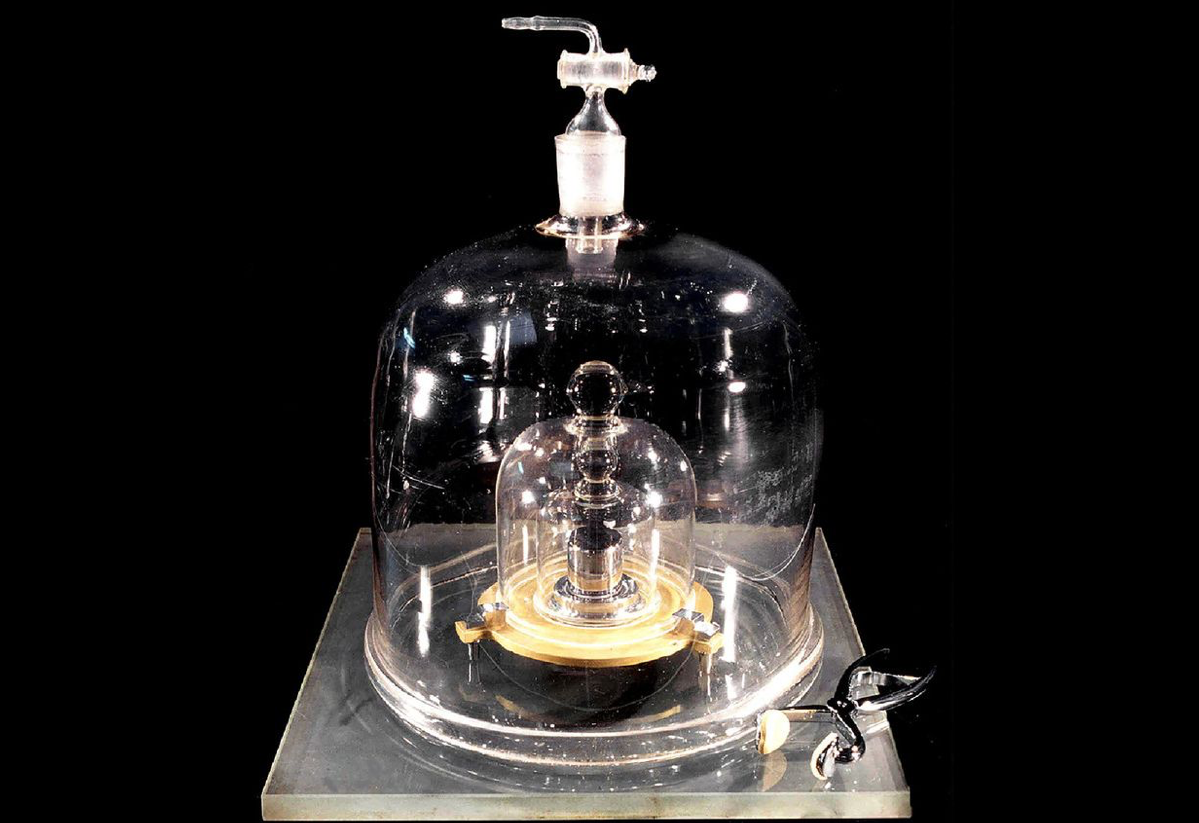
\includegraphics[scale=0.09]{./images/1kg}
\end{figure}
\pause

\textbf{forza} $(N = kg \ m / s^2 )$: Seconda Legge di Newton 
$$\vec{F} = m \  \vec{a}$$ 
\pause

\textbf{forza di gravità}: La forza di gravità (forza peso, o più semplicemente peso) è, in fisica classica, la forza che un campo gravitazionale (ad esempio quello terrestre) esercita su un corpo avente massa.
\pause

$$\vec{F_{grav}} = m \  \vec{g}, \ \ dove \  \vec{g} = 9.81 (m/s^2)$$ 
\end{frame}

\begin{frame}
\textbf{centro di massa} $(m)$: in meccanica classica, il centro di massa (o centro di gravità, o baricentro) di un sistema è il punto geometrico corrispondente al valor medio della distribuzione della massa del sistema nello spazio.
\pause

\begin{figure}
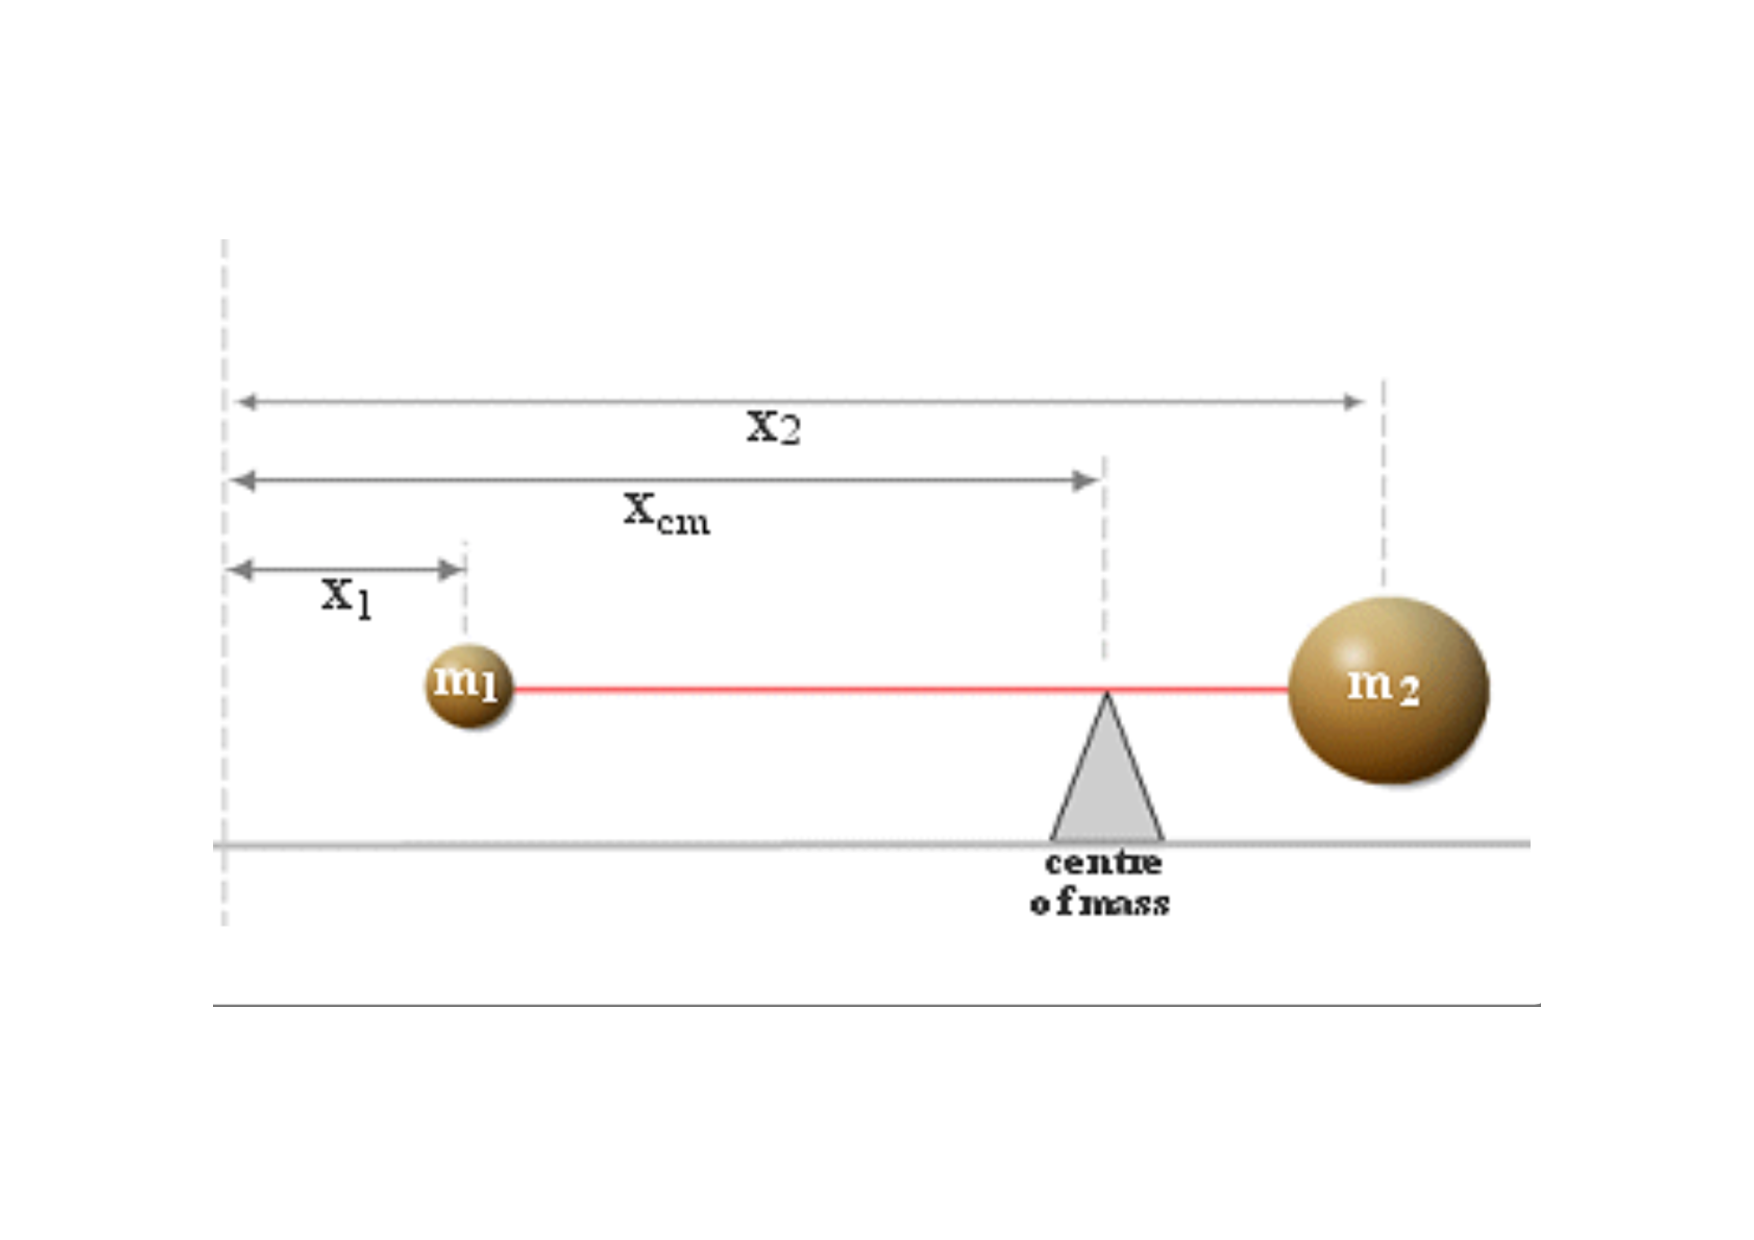
\includegraphics[scale=0.25]{./images/cdm}
\end{figure}
$$x_{cm} (m_1 + m_2) = x_1 m_1 + x_2 + m_2$$ \\
\pause

$$x_{cm}  = \frac{x_1 m_1 + x_2 + m_2}{(m_1 + m_2)}$$
\end{frame}
\section{Massa vs Momento d'Inerzia}
\end{document}
